\chapter{Análise de Resultados}
\label{cap:resultados}
%Neste capítulo são apresentados os resultados encontrados a partir dos três experimentos efetuados.%Primeiro são apresentados os resultados encontrados  nos três experimentos, sendo assim feita uma análise da interferência nos mesmos. Em seguida é feita uma análise estatistica do experimento três sendo assim abordada, a questão da predição de desempenho

\section{Interferência de Desempenho}
O primeiro experimento teve como intuito observar se de fato havia algum tipo de interferência significativa durante a execução de aplicações em máquinas virtuais concorrentes. Para isso, foram selecionadas as seguintes ferramentas: \textit{bzip2}, \textit{grep}, \textit{povray}, \textit{crypt} e \textit{cp} para calculo da degradação. A Figura \ref{first_experiment} apresenta os resultados para esse conjunto de aplicações, utilizando a equação \ref{eq:combined}. 

\begin{figure}[!htb]
\centering
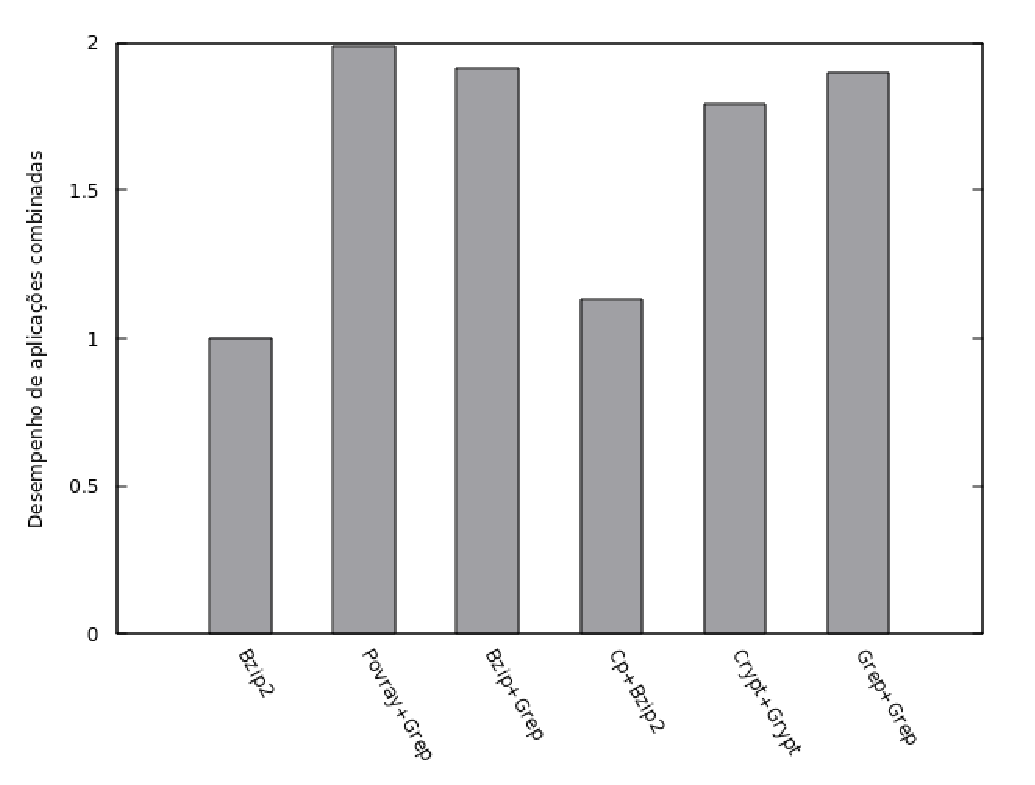
\includegraphics [keepaspectratio=true,scale=0.65]{graficos/exp1.eps}
\caption{Pontuação combinada de aplicações selecionadas para o primeiro experimento}
\label{first_experiment}
\end{figure} 

Levando-se em conta que cada aplicação consome exatamente metade dos recursos computacionais, o desempenho esperado seria 1. Entretanto, por conta da variação de interferência dada a combinação de aplicações, o desempenho também muda. Desse modo, aplicações que raramente interferem no desempenho uma da outra, a pontuação se aproxima de 2. Em contrapartida, aplicações que interferem substancialmente uma na outra, sua pontuação tende a ser baixa. Os resultados apresentados neste experimento, mostram por exemplo que \textit{povray+grep} apresentam um grau de interferência praticamente nulo, enquanto que \textit{cp + bzpip} o grau de interferência é maior a ponto da pontuação se aproximar de 1. Desse modo, era de se esperar, que dados os resultados referentes a interferência de aplicações apresentados no trabalho de \citeonline{koh2007}, que o desempenho combinado de aplicações iguais caísse drasticamente. Uma das hipóteses é que a configuração de \textit{hardware} utilizada neste trabalho, típica para ambientes em produção, minimiza o grau de degradação de algumas aplicações, mesmo quando executadas contra elas mesmas em máquinas virtuais diferentes. Em específico, foi utilizado nesse servidor uma configuração de redundância de disco \textit{RAID 5}, o que pode minimizar ainda mais a degradação de desempenho para aplicações com perfis de \textit{Entrada/Saida} como \textit{Grep} e \textit{Crypt}.

%Segundo \citeonline{koh2007}, uma aplicação executando sem qualquer máquina virtual concorrente, possui os benefícios de se aproveitar da velocidade mais alta da memória \textit{cache} obtendo dessa forma ganhos de desempenho. Em contrapartida, com outra máquina virtual em execução concorrente em um mesmo servidor, durante a execução de uma aplicação o \textit{hypervisor} pode mudar para outra máquina virtual (no final de um \textit{quantum}). Sendo a \textit{cache} então agora utilizada por outra máquina virtual. Ao voltar para máquina virtual de origem, é bastante provável que a  \textit{cache} esteja inutilizável. Outro problema que \citeonline{koh2007} cita é que é bastante difícil de prever e tratar esse tipo de problema dado que as máquinas virtuais não possuem informações sobre as mudanças de contexto feitas pelo \textit{hypervisor}, e nem mesmo os próprios \textit{hypervisors} possuem informações sobre as aplicações que estão sendo executadas nas máquinas virtuais.

Um dos receios era que os procedimentos definidos na metodologia não fossem suficientes, dada a configuração de \textit{hardware} do servidor, para observar a degradação de desempenho das aplicações. Entretanto, os resultados desse experimento demonstraram que com esses procedimentos é possível observar um grau de interferência para um conjunto de aplicações. O próximo passo então foi observar o grau de interferência para um conjunto maior de aplicações afim de observar padrões de interferências dado o perfil de execução das aplicações ( disco, \textit{cpu} e memória).

\section{Desempenho contra diferentes tipos de Aplicações}
\label{sec:exp2}
No segundo experimento foi construída uma matriz \textit{nxn} com as combinações possíveis das aplicações sendo executadas tanto quanto \textit{Background } como \textit{Foreground}. Desse modo, contou-se com mais combinações de resultados sendo possível observar se existia ou não um padrão de degradação dado o tipo de aplicação que estava sendo executada. A figura \ref{second_experiment} apresenta esses resultados. %Para apresentação desses resultados, foram selecionadas as ferramentas que tiveram resultados mais significativos seja no sentido de ter proporcionado interferência ou não. A figura \ref{second_experiment} apresenta esses resultados.

\begin{figure}[!h]
\centering
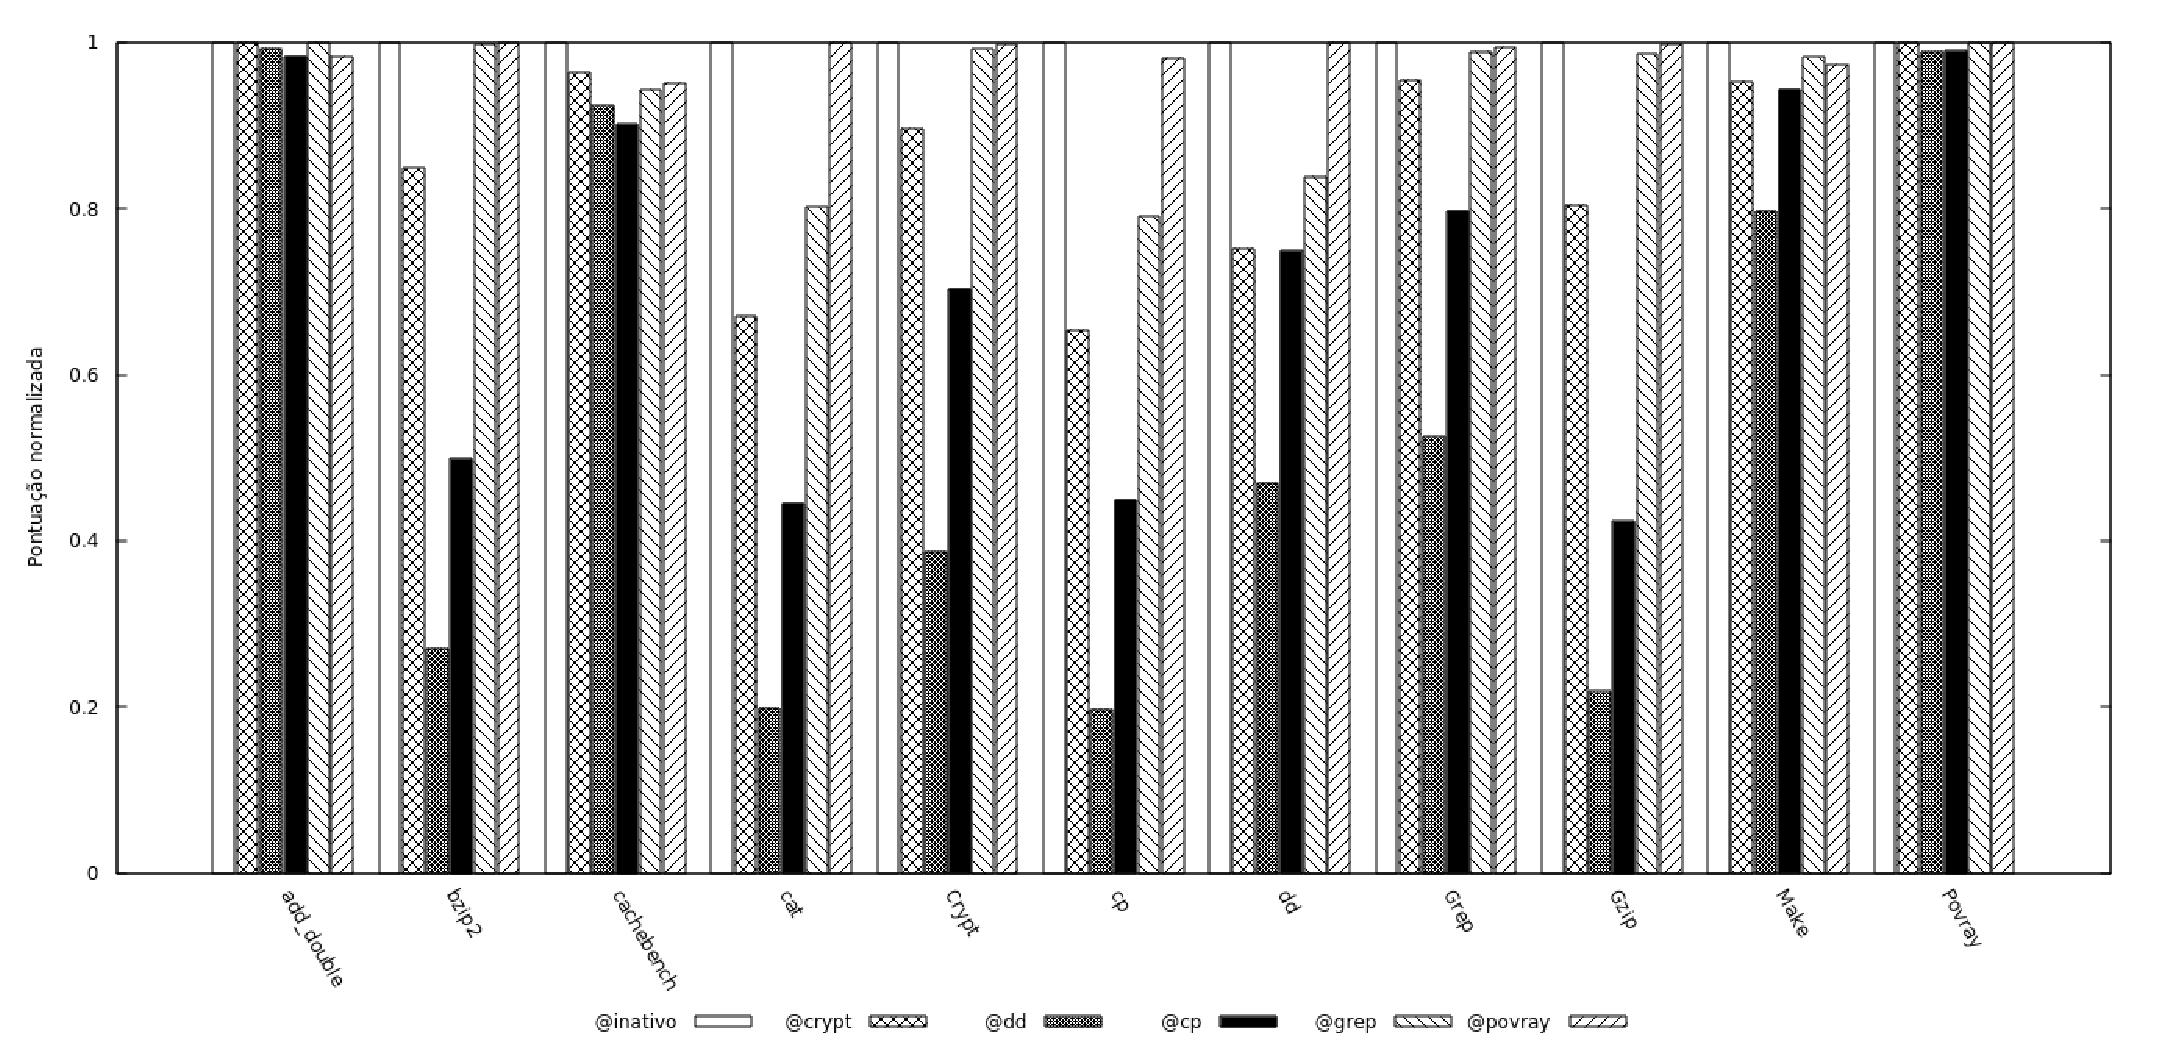
\includegraphics [keepaspectratio=true,scale=0.45]{graficos/exp_2_foreground.eps}
\caption{Pontuação normalizada contra um conjunto de aplicações}
\label{second_experiment}
\end{figure} 

Os resultados desse segundo experimento mostram que de maneira geral algumas aplicações tendem a sofrer e a causar menos interferência do que outras aplicações. É o caso de \textit{add\_double}, \textit{cachebench}, \textit{make} e \textit{povray}. Não por acaso, são ferramentas que não possuem perfis de cargas de trabalho voltados para operações de \textit{entrada/saída} ( \textit{add\_double} possui perfil voltado para \textit{cpu}, \textit{make} e \textit{povray} possuem perfil misto mas mais voltado para operações em \textit{cpu} do que de \textit{entrada/saída} e \textit{cachebench} é mais voltado para operações no sistema de memória). 

Assim, nota-se que essas aplicações, por possuírem um perfil de carga de trabalho voltado mais para \textit{cpu} e memória (no caso do \textit{cachebench}), praticamente não interferem em aplicações que possuem um perfil voltado para \textit{operações de entrada/saída} e nem mesmo sofrem interferência significativa desse tipo de aplicações. Como pode ser observado, por exemplo, os resultados apresentados na execução de \textit{povray} contra um conjunto de ferramentas, na Figura \ref{second_experiment}. Nota-se que a pontuação de \textit{povray} contra esse conjunto de aplicações ficou próxima de 1 o que indica o grau de interferência bastante insignificante, o mesmo ocorrendo com \textit{add\_double}.

No caso do \textit{cachebench}, mesmo tendo sido uma das ferramentas que menos sofreu interferência, percebe-se um grau de interferência mais elevado do que das outras duas (\textit{povray} e \textit{add\_double}), isso se deve ao fato que o sistema de memória acaba atuando principalmente em operações de \textit{cache} tanto em aplicações com perfil voltado para \textit{cpu} quanto em aplicações com perfil voltado para operações de \textit{entrada/saída}.

Para o restante das aplicações, observa-se um grau de interferência maior e com mais variações dependendo da aplicação que está sendo executada em \textit{background}. Essas aplicações, são típicas aplicações de \textit{entrada/saída}, com suas cargas de trabalho atuando em operações de escrita ou leitura em disco. Observa-se por exemplo, que \textit{dd} e \textit{cp} são as aplicações que causam maior degradação no desempenho das aplicações voltadas para \textit{entrada/saída}. Dessa forma  em uma das combinações apresentadas mostra que, executando \textit{Bzip2} contra \textit{dd}, a pontuação fica abaixo de 0.4, evidenciando um elevado grau de degradação.

Dada a variação de interferência de desempenho entre essas aplicações, vale ressaltar alguns casos. Entre eles, destaca-se por exemplo que a pontuação alcançada de \textit{gzip} e \textit{bzip2} contra \textit{grep} indica um grau de degradação de desempenho pequeno ou praticamente nulo. Em contrapartida, a pontuação alcançada por \textit{cp}, \textit{cat} e \textit{dd} contra \textit{grep}, mostram uma degradação do desempenho maior se comparada com \textit{gzip} e \textit{bzip2} contra \textit{grep}. Indicando, dessa forma que mesmo dentre as aplicações típicas de \textit{entrada/saída} pode haver um padrão de interferência dado o seu tipo de execução( escrita ou leitura). 

\begin{figure}[!h]
\centering
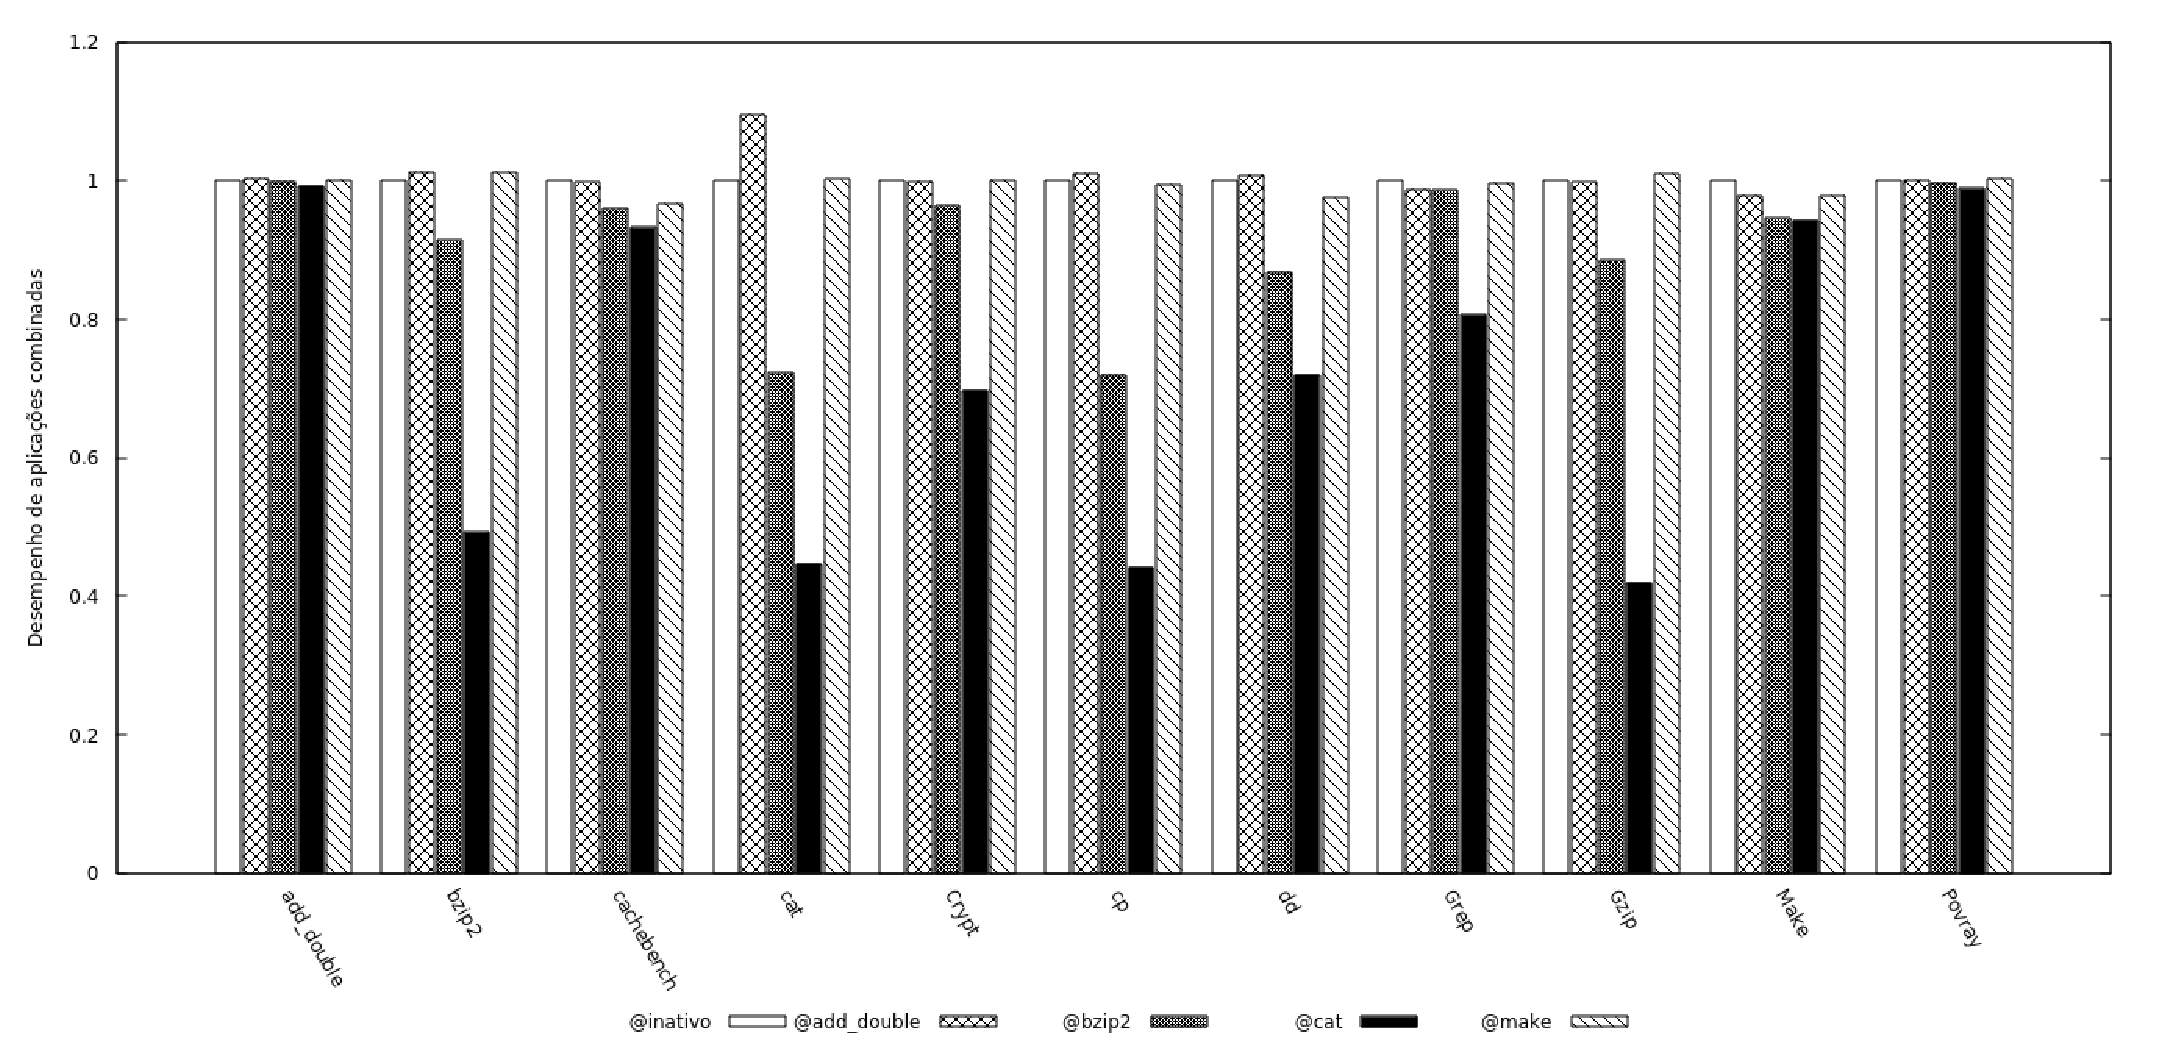
\includegraphics [keepaspectratio=true,scale=0.45]{graficos/exp_2_1_foreground.eps}
\caption{Variação de desempenho para um conjunto de aplicações}
\label{second_experiment_second}
\end{figure} 

A Figura \ref{second_experiment_second} apresenta os resultados de interferência para um outra combinação de aplicações. Nota-se que mesmo executando \textit{add\_double}@\textit{add\_double} a interferência apresentada é praticamente inexistente, evidenciando assim que as cargas de trabalhos aplicados para \textit{cpu} não estavam sendo suficientes para que algum tipo de interferência fosse observável. Mais uma vez, nota-se maior degradação no desempenho geral em aplicações que possui um perfil de \textit{entrada/saída}.

Os resultados deste segundo experimento demonstraram que o perfil de execução de aplicação influenciam de maneira considerável no desempenho de uma aplicação que está sendo executada em uma outra máquina virtual. Observa-se que a tendência é que aplicações com perfil voltadas para uso de disco sofram pouca interferência de aplicações com perfil de uso mais voltado para \textit{cpu} e memória. Em contrapartida, seus desempenhos caem consideravelmente quando executadas contra outras aplicações com perfil de uso voltado para disco. Uma hipótese levantada neste experimento é pode haver um padrão de degradação dado o tipo de operação de disco ao qual as aplicações são voltadas (leitura ou escrita). Com esses resultados, chegou-se a conclusão que os testes definidos para \textit{cpu} são insuficientes para que se observe algum tipo de degradação nesse perfil de execução. 
% Além disso, nota ferramentas quando executadas contra ferramentas com o mesmo perfil de execução (\textit{cpu} x \textit{cpu}), demonstram uma interferência insignificante. 

\section{Interferência nas Métricas de Desempenho a nível de Sistema}
O terceiro experimento consistiu em coletar os dados referentes as métricas de desempenho a nível desse sistema. Desse modo, foi possível observar o perfil de execução das aplicações bem como avaliar como ocorre o impacto da degradação do desempenho nesses tipos de métricas. Como observado no experimento 2, algumas aplicações sofreram pouca degradação em seus desempenhos bem como interferiu muito pouco contra outras aplicações. Dessa forma, optou-se por restringir esse experimento às ferramentas aos quais foram observados o grau de interferência maior, sendo removidas então deste terceiro experimento \textit{make}, \textit{povray}, \textit{add\_double} e \textit{cachebench}.

\begin{figure}[!h]
\centering
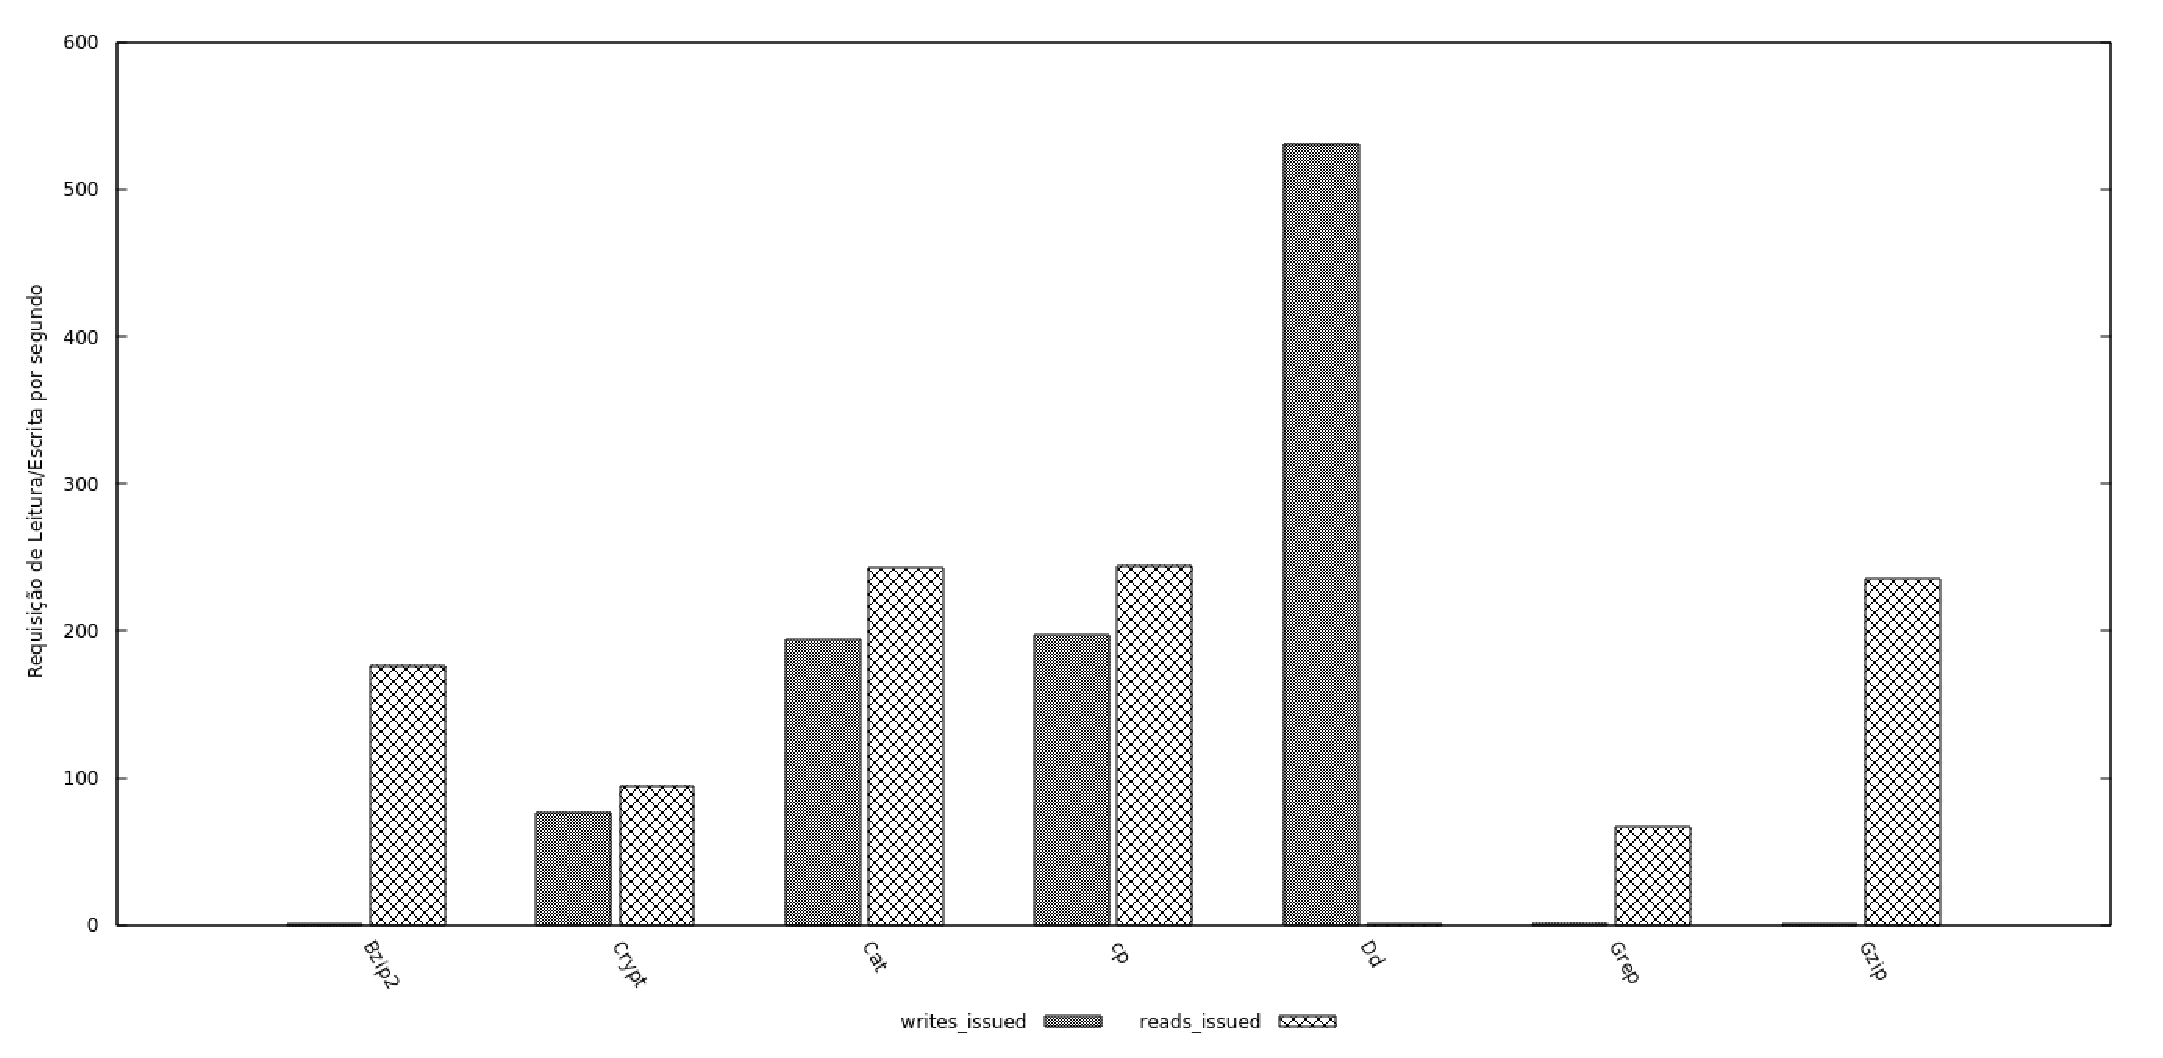
\includegraphics [keepaspectratio=true,scale=0.4]{graficos/exp_3_read_write.eps}
\caption{Desempenho alcançado das aplicações para requisções de escrita e leitura em disco}
\label{disk_operations}
\end{figure} 

\begin{figure}[!h]
\centering
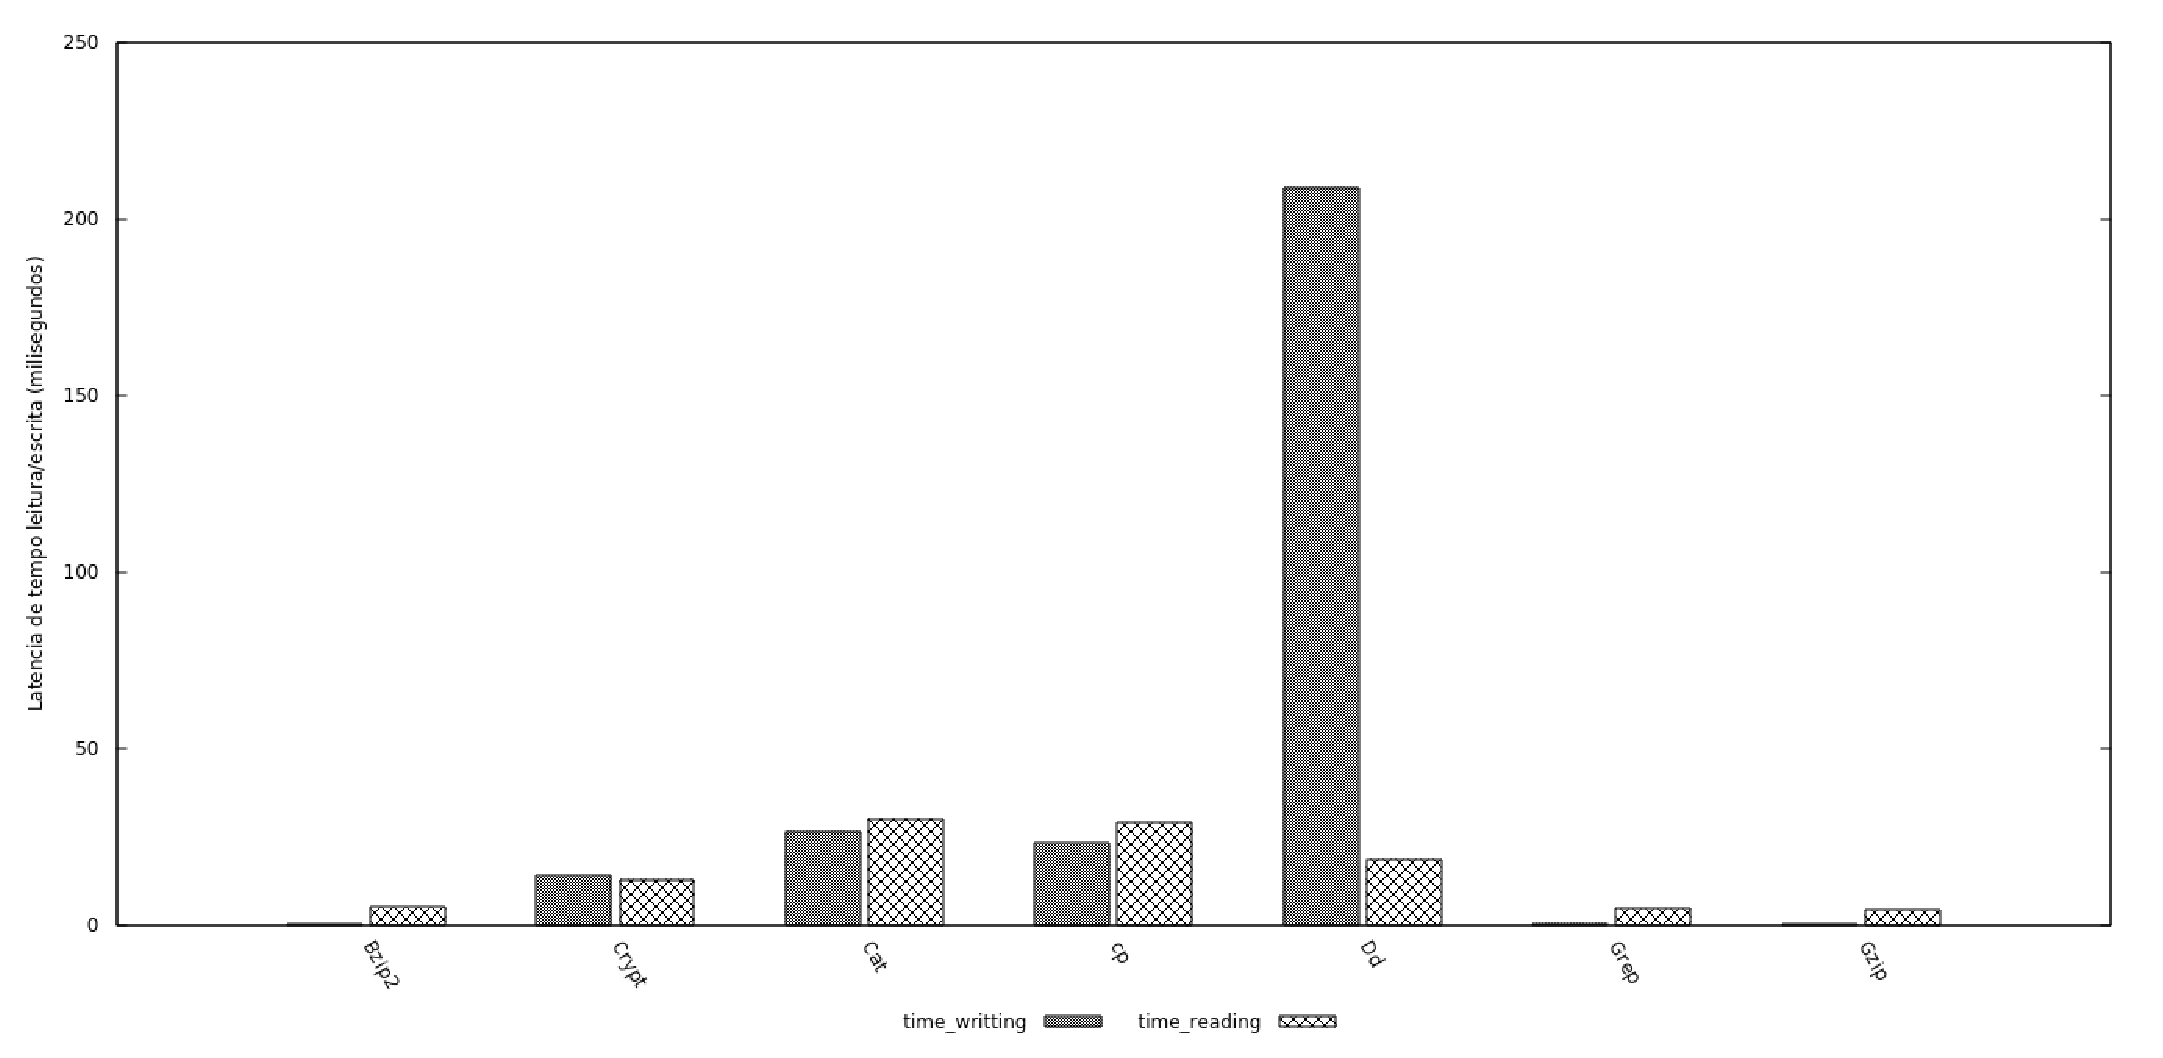
\includegraphics [keepaspectratio=true,scale=0.4]{graficos/exp2_latency.eps}
\caption{Tempo que as aplicações levam para executar uma operação de leitura e escrita em disco}
\label{latency_disk}
\end{figure}

\begin{figure}[!h]
\centering
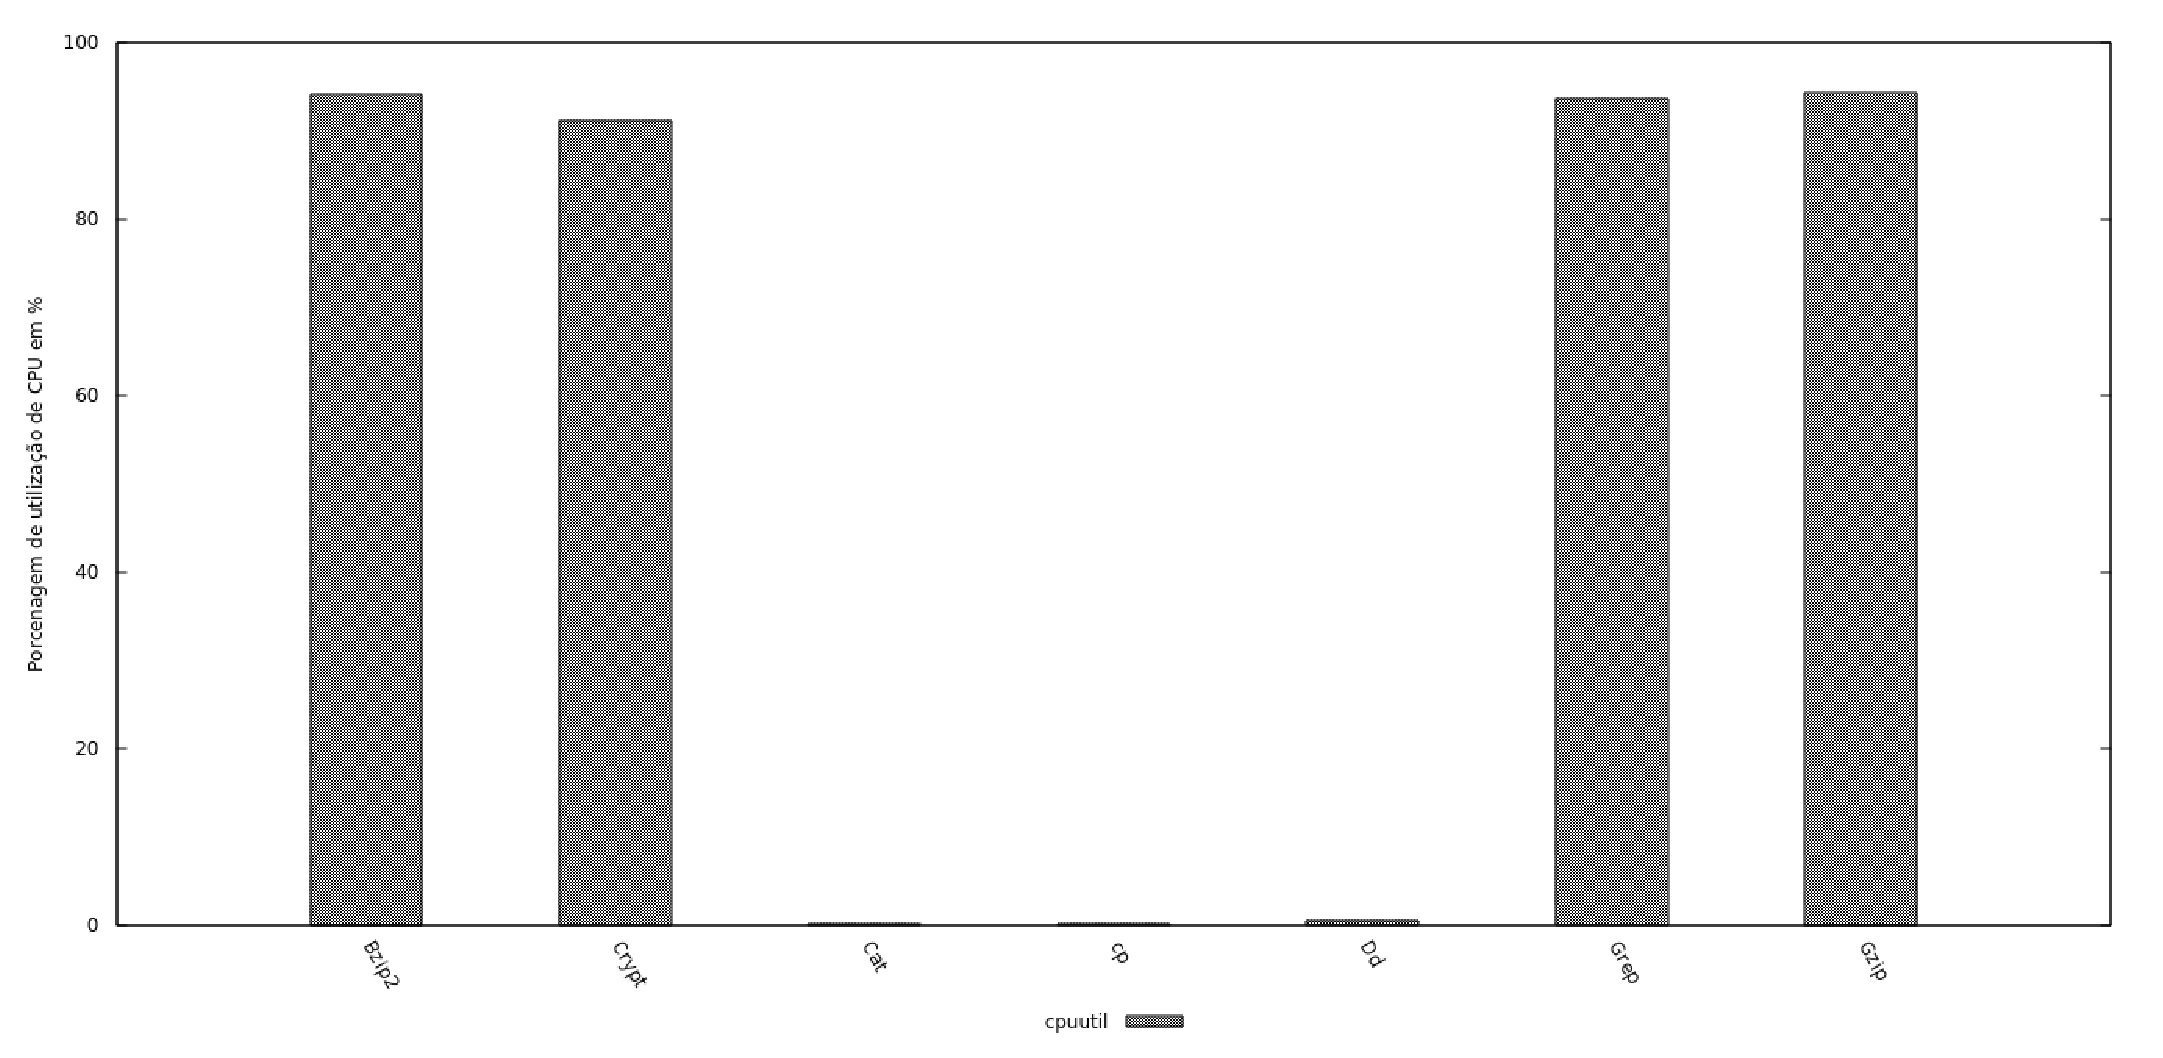
\includegraphics [keepaspectratio=true,scale=0.4]{graficos/exp_3_cpu.eps}
\caption{Porcentagem de utilização de cpu para cada aplicação}
\label{cpu_util}
\end{figure}  

As imagens \ref{disk_operations}, \ref{latency_disk} e \ref{cpu_util} mostram o desempenho das aplicações quando executadas contra um servidor inativo. Os dados apresentados permitem observar o perfil de execução de algumas aplicações a partir da pontuação alcançada nas métricas de desempenho a nível de sistema. Percebe-se dessa forma que aplicações como \textit{crypt}, \textit{cat}, \textit{cp} possui um perfil misto nas operações em disco, ou seja, executam de forma quase igualitária tanto operações de leitura quanto operações de escrita em disco. Em contrapartida, aplicações como \textit{dd}, \textit{grep}, \textit{gzip} e \textit{Bzip2} possuem um perfil único no que tange as operações em disco, com \textit{dd} tendo uma elevada pontuação para operações de escrita de disco, e as outras três possuindo um perfil voltado mais para leitura em disco. O perfil de execução dessas aplicações para as métricas de leitura e escrita em disco reflete o perfil para o tempo de escrita e de leitura em disco, mantendo dessa forma, o mesmo padrão de desempenho para essas duas últimas métricas. Para porcentagem de utilização de \textit{cpu}, observa-se que as aplicações \textit{bzip2}, \textit{crypt}, \textit{grep} e \textit{gzip} possui taxas elevadas de utilização de \textit{cpu}, mostrando assim um  perfil misto de execução com relação à utilização de \textit{cpu} e \textit{disco}. Já \textit{cat}, \textit{cp} e \textit{dd} apresentam baixas taxas de utilização de \textit{cpu} evidenciando dessa forma seu perfil voltado para utilização de disco.

No experimento 2 observou-se que algumas aplicações podem sofrer maior degradação dependendo da aplicação que está sendo executada como \textit{background}. \textit{Bzip2}, por exemplo, obteve uma queda de desempenho acentuada executando contra \textit{cp}, \textit{cat} e \textit{dd}. Já contra \textit{Grep} e \textit{crypt}, obteve pontuação relativamente alta. A Figura \ref{bzip_performance} mostra como se dá essa degradação nas métricas a nível de sistema de \textit{bzip2} contra um conjunto de aplicações. 
%Para avaliar como cada aplicação interfere na outra foi utilizada a pontuação normalizada para cada métrica a nível de sistema. Desse modo  a seguir são apresentados algumas combinações de execução concorrente. %Um dos problemas enfrentados é a pequena variabilidade durante a coleta de dados. Assim, notou-se que as métricas que sofrem uma degradação nula  durante a execuçao contra uma determinada aplicaçao em outra maquina virtual pode a vir a ter seu desempenho   
\begin{figure}[!h]
\centering
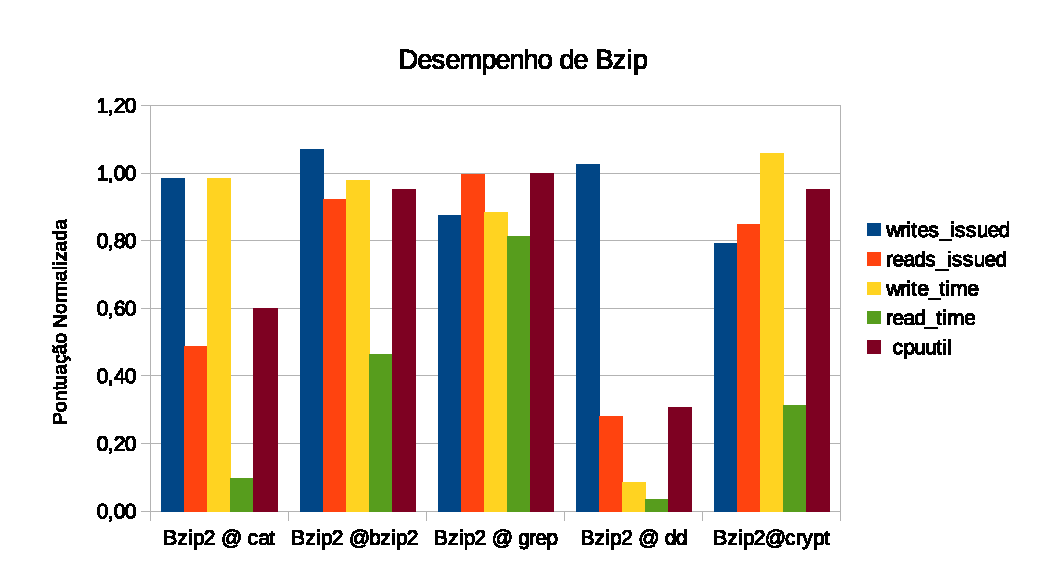
\includegraphics [keepaspectratio=true,scale=0.8]{graficos/bzip_performance.eps}
\caption{Pontuação normalizada das métricas a nível de sitema de \textit{Bzip2} contra diferentes tipos de aplicações.}
\label{bzip_performance}
\end{figure}  

As pontuações normalizadas de algumas métricas ultrapassam o valor de 1, o que teoricamente seria impossível dado que o desempenho, contra uma aplicação \textit{background}, tende a ser menor ou igual a 1 dependendo da aplicação. Entretanto, as medições \textit{F@B} e \textit{F@Inativo} são feitas em experimentos diferentes. Dessa forma, observou-se que, mesmo coletando uma amostra de 300 valores para cada métrica, pode haver uma pequena variação de experimento para experimento. Assim, uma pontuação de uma métrica que não sofre degradação contra uma determinada aplicação \textit{background} (F@B), pode naquele momento alcançar um valor um pouco maior do que quando foi executando contra uma máquina virtual inativa (F@Inativo), resultando em uma pontuação normalizada maior que 1 de acordo com a equação \ref{eq:degradation}.

Nota-se, portanto, que \textit{bzip2} contra \textit{cat} resulta uma interferência nula na métrica \textit{writes\_issued}, dada a pontuação normalizada desta, por outro lado a pontuação normalizada de \textit{cpuutil}, \textit{writes\_issued} e \textit{read\_time} caíram drasticamente. A queda de \textit{cpuutil} em \textit{bzip2}, mesmo com \textit{cat} possuindo baixa taxa de utilização de \textit{cpu}, pode ser explicada pela pontuação alcançada por \textit{read\_time}. Uma pontuação normalizada de \textit{read\_time} mais baixa indica que \textit{bzip2} agora está levando mais tempo para realizar poucas requisições de disco, fazendo que a \textit{cpu} fique mais tempo ociosa esperando por operações de \textit{entrada/saída}. Por possuir um perfil mais voltado para operações de leitura em disco, o desempenho de \textit{bzip2} tende a ser fortemente influenciado com a queda de valores de \textit{reads\_issued} e \textit{read\_time}.

Executando \textit{Bzip2}, \textit{grep} e \textit{crypt} como \textit{background}, \textit{Bzip2} tende a ter um desempenho melhor, tendo apenas como maior degradação a métrica \textit{reads\_issued}, sendo possivelmente a causa da pequena degradação sofrida por \textit{Bzip2} quando executado contra essas aplicações, como apresentado nas imagens \ref{second_experiment} e \ref{second_experiment_second}. Com \textit{dd} como \textit{background}, \textit{Bzip2} possui uma degração em seu desempenho semelhante à quando executada contra \textit{cat}. Novamente, têm-se uma queda acentuada nas pontuações normalizadas de \textit{cpuutil}, \textit{reads\_issued} e \textit{read\_time}.

A Figura \ref{dd_performance} apresenta a variação da degradação sofrida por \textit{dd} para cada tipo de métrica. \textit{cp} possui uma degradação de desempenho semelhante tanto para as aplicações com perfis mistos  quanto para aplicações voltadas para operações em disco, com exceção do caso de quando ele é executado contra ele mesmo. Sua pontuação, como apresentado nas imagens \ref{second_experiment_second} e \ref{second_experiment}, fica na faixa de 0.7 \char`\~  0.85 contra aplicações de perfil misto e de disco e próximo de 0.5 quando executado contra ele mesmo, e isso se reflete em suas métricas. Principalmente \textit{writes\_issued}, que mantém esse mesmo padrão de degradação evideciando dessa forma que o desempenho de \textit{dd} é fortemente influenciado por essa métrica, visto que, \textit{dd} possui um perfil voltado para escrita de disco.
 
\begin{figure}[H]
\centering
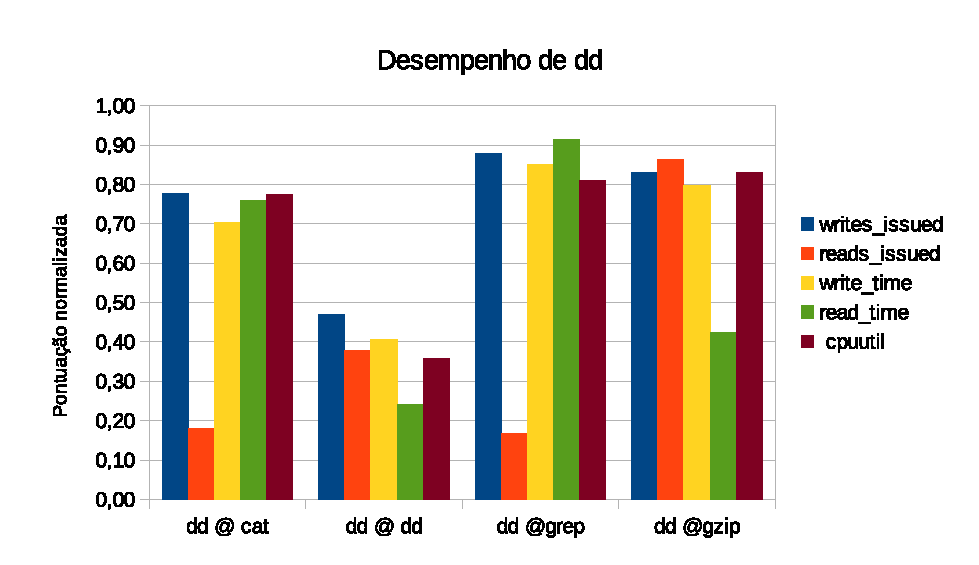
\includegraphics [keepaspectratio=true,scale=0.7]{graficos/dd_performance.eps}
\caption{Pontuação normalizada das métricas a nível de sitema de \textit{dd} contra diferentes aplicações.}
\label{dd_performance}
\end{figure}  


A Figura \ref{grep_performance} apresenta a degradação sofrida por \textit{grep} em suas métricas indicadoras de desempenho para cada aplicação. Observa-se que mais uma vez, que o desempenho de uma aplicação é determinado pelo grau de degradação sofrido pela sua métrica de maior uso. Assim, executando \textit{grep} contra \textit{dd}, sua pontuação normalizada de \textit{writes\_issued} alcança 0.76 enquanto que \textit{reads\_issued} atinge 0.54 e, levando-se em conta seu tempo de execução, a pontuação atinge 0.52 como mostrado na Figura \ref{second_experiment}, evidenciando que a degradaçao sofrida por \textit{grep} advém de valores de \textit{reads\_issued} mais baixos. Nota-se, também que \textit{grep} tem maiores perdas de desempenho para \textit{reads\_issued} quando executado contra, \textit{cp}, \textit{cat} e \textit{dd} do que contra \textit{Bzip2} e \textit{crypt}. Isso se deve ao fato de que as três primeiras aplicações geram mais requisições de disco ( leitura e escrita) do que as duas últimas.

\begin{figure}[H]
\centering
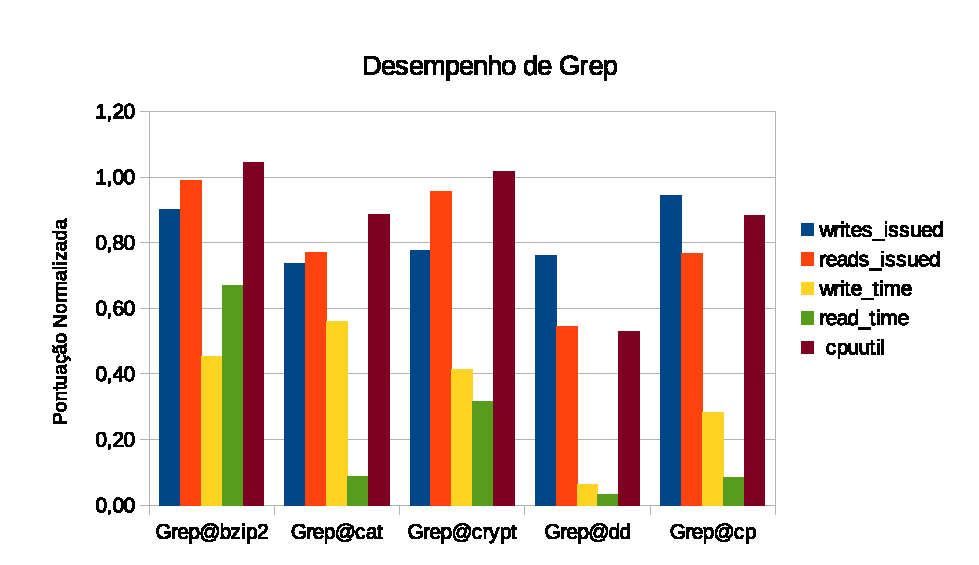
\includegraphics [keepaspectratio=true,scale=0.8]{graficos/grep_performance.eps}
\caption{Pontuação normalizada das métricas a nível de sitema de \textit{Grep} contra diferentes aplicações.}
\label{grep_performance}
\end{figure}   

Com os resultados deste experimento foi possível traçar um perfil de execução para cada ferramenta, bem como observar como o seu perfil de execução influencia bastante em seu desempenho final quando executado contra uma aplicação em \textit{background}. Uma das hipóteses levantadas na Seção \ref{sec:exp2} era de que poderia haver uma padrão de degradação dentre as aplicações com perfil voltado para operações de disco. Com os resultados apresentados tal hipótese não pode ser confirmada dado que o se observou foi que o que causa maior degradação para esse conjunto de aplicações são as taxas mais elevadas de requisições no disco que uma aplicação \textit{background} pode gerar. De maneira geral, percebe-se que aplicações que possuem perfil misto para \textit{cpu} e \textit{disco}, possuem baixa degradação contra aplicações de perfil misto e de perfil voltado para \textit{cpu}, e uma elevada perda de desempenho quando executadas contra aplicações de perfil apenas de disco. Aplicações com perfil de disco possuem baixa degradação apenas quando executadas contra aplicações de perfil \textit{cpu}. 

\section{Predição de Desempenho}
\label{sec:performance_predict}
%\begin{figure}[!h]
%\centering
%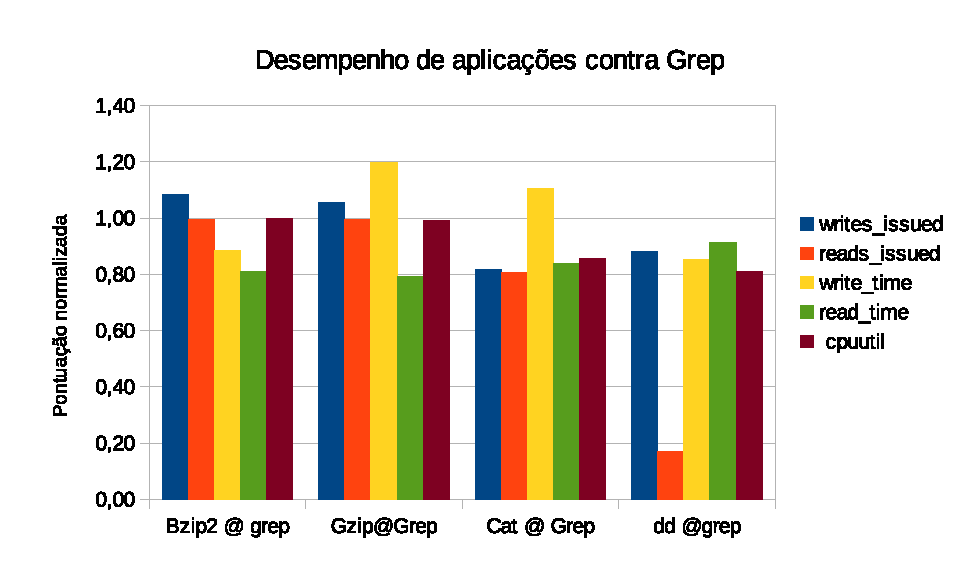
\includegraphics [keepaspectratio=true,scale=1.0]{graficos/comparative_performance.eps}
%\caption{Comparativo de desempenho de \textit{Bzip2}, \textit{Gzip}, \textit{Cat} e \textit{dd} contra \textit{Grep}.}
%\label{comparative_performance}
%\end{figure}   


 %Entretanto, os resultados de \textit{grep+grep} e \textit{crypt+crypt} mostram que mesmo aplicações iguais podem não interferir tanto quanto o esperado. Uma das hipóteses iniciais é de que configuração de disco em \textit{raid 5} do servidor, minimiza a interferência para aplicações com perfis de \textit{Entrada\Saída} como \textit{Grep} e \textit{Crypt}. Outro fator que 

  

%Análise da interferencia
%primeiro experimento
%segundo experimento
%Terceiro experimento
%características a nível de sistema
